\section*{前言}
我们很自豪地向您介绍第四版《大规模并行处理器编程:实践方法》。

结合了多核 CPU 和多线程 GPU 的大众市场计算系统为笔记本电脑带来了万亿级计算,为集群带来了百亿亿级计算。 
有了这样的计算能力,我们正处于科学、工程、医学和商业学科中广泛使用计算实验的黎明。 
我们还见证了 GPU 计算在金融、电子商务、石油和天然气以及制造等关键行业垂直市场中的广泛采用。 
这些学科的突破将通过使用规模、准确性、安全性、可控性和可观察性达到前所未有的水平的计算实验来实现。 
本书为这一愿景提供了一个关键要素:向数百万研究生和本科生教授并行编程,以便计算思维和并行编程技能将像微积分技能一样普及。

本书的主要目标读者包括所有科学和工程学科的研究生和本科生,这些学科需要计算思维和并行编程技能才能取得突破。 
本书还被需要更新并行计算技能并跟上不断增长的技术发展速度的行业专业开发人员成功使用。 
这些专业开发人员的工作领域包括机器学习、网络安全、自动驾驶汽车、计算金融、数据分析、认知计算、机械工程、
土木工程、电气工程、生物工程、物理、化学、天文学和地理学,他们使用计算 来推进他们的领域。 
因此,这些开发人员既是各自领域的专家,又是程序员。 本书采用通过建立对技术的直观理解来教授并行编程的方法。 
我们假设读者至少有一些基本的 C 编程经验。 我们使用 CUDA C,这是 NVIDIA GPU 支持的并行编程环境。 
消费者和专业人士手中有超过 10 亿个这样的处理器,超过 40 万程序员正在积极使用 CUDA。 
作为学习体验的一部分,您将开发的应用程序将可由非常大的用户社区运行。

自2016年第三版出版以来,我们收到了读者和讲师的大量评论。 他们中的许多人告诉我们他们看重的现有功能。 
其他人给了我们一些关于如何扩展这本书的内容以使其更有价值的想法。 
此外,自2016年以来,异构并行计算的硬件和软件都取得了巨大的进步。在硬件领域,自第三版以来又推出了三代GPU计算架构,
即Volta、Turing和Ampere。 在软件领域,CUDA 9 到 CUDA 11 允许程序员访问新的硬件和系统功能。 
新的算法也已被开发出来。 因此,我们添加了四个新章节并重写了大量现有章节。

新增的四个章节包括一个新的基础章节,即第 4 章(计算架构和调度),以及三个新的并行模式和应用章节:第 8 章(模板)、第 10 章(减少和最小化发散)和第 13 章( 排序)。 我们添加这些章节的动机如下:

\begin{itemize}
	\item 第4 章(计算架构和调度):在上一版本中,有关架构和调度注意事项的讨论分散在多个章节中。 
		在本版中,第 4 章将这些讨论整合为一个重点章节,为对此主题特别感兴趣的读者提供集中参考。

	\item 第8 章(模板):在上一版本中,鉴于两种模式之间的相似性,在卷积章节中简要提到了模板模式。 
		在这个版本中,第 8 章对模板模式进行了更彻底的处理,强调了计算背后的数学背景以及使其不同于卷积的方面,
		从而实现了额外的优化。 本章还提供了处理三维网格和数据的示例。

	\item 第10 章(减少和最小化发散):在上一版本中,在性能注意事项章节中简要介绍了减少模式。 
		在本版本中,第 10 章更完整地介绍了缩减模式,并采用增量方法应用优化,并对相关性能权衡进行了更彻底的分析。

	\item 第13 章(排序):在上一版本中,在有关合并模式的章节中简要提到了合并排序。 
		在本版本中,第 13 章将基数排序介绍为一种非比较排序算法,该算法非常适合 GPU 并行化,
		并遵循增量方法来优化它并分析性能权衡。 本章还讨论了合并排序。
\end{itemize}

除新增章节外,所有章节均进行了修订,部分章节进行了大幅重写。 这些章节包括以下内容:

\begin{itemize}
	\item 第 6 章(性能注意事项):本章之前的一些架构注意事项已移至新的第 4 章,并且缩减示例移至新的第 10 章。
		取而代之的是,本章被重写以提供更全面的说明。 处理线程粒度注意事项,更值得注意的是,
		提供常见性能优化策略和每个策略解决的性能瓶颈的清单。 当我们优化代码以实现各种并行模式和应用程序时,
		在教科书的其余部分中都会引用此清单。 目标是强化系统性和增量式方法来优化并行程序的性能。

	\item 第7 章(卷积):在上一版本中,有关卷积模式的章节使用一维卷积作为运行示例,最后简要处理了二维卷积。 
		在这个版本中,本章被重写,从一开始就更多地关注二维卷积。 这一变化使我们能够解决高维平铺的复杂性和复杂性,
		并为读者在第 16 章中学习卷积神经网络提供更好的背景知识。

	\item 第9 章(并行直方图):在上一版本中,有关直方图模式的章节从一开始就应用了线程粗化优化,
		并将私有化优化与共享内存的使用相结合。 在本版本中,本章被重写,以遵循更加渐进的性能优化方法。 
		现在提出的初始实现不应用线程粗化。 私有化和私有容器的共享内存的使用被区分为两个单独的优化,
		前者旨在减少原子争用,后者旨在减少访问延迟。 线程粗化是在私有化之后应用的,
		因为粗化的一个主要好处是减少提交给公共副本的私有副本的数量。 
		本章的新组织与全书遵循的系统和增量性能优化方法更加一致。 
		我们还将这一章移到了有关缩减和扫描模式的章节之前,以便更快地介绍原子操作,因为它们用于多块缩减和单遍扫描内核。

	\item 第14 章(稀疏矩阵计算):在本版本中,本章被重写,以遵循更系统的方法来分析不同稀疏矩阵存储格式之间的权衡。 
		本章开头介绍了设计不同稀疏矩阵存储格式时需要考虑的一系列注意事项。 
		然后在整个章节中使用这个设计考虑因素列表来系统地分析不同格式之间的权衡。

	\item 第15 章(图遍历):在上一版本中,图遍历的章节重点介绍了特定的BFS 并行化策略。 
		在本版本中,本章进行了显着扩展,涵盖了一组更全面的替代并行化策略,并分析了它们之间的权衡。 
		除了原始实现(即基于顶点中心推、基于边界的实现)之外,
		这些策略还包括基于顶点中心推、基于顶点中心拉、以边为中心和线性代数实现。 
		这些替代方案的分类并非 BFS 所独有,而是普遍适用于并行图算法。

	\item 第16 章(深度学习):在本版本中,本章被重写,为理解现代神经网络提供全面而直观的理论背景。 
		背景知识使读者更容易全面理解神经网络的计算组件,例如全连接层、激活层和卷积层。 
		它还消除了理解训练卷积神经网络的核函数的一些常见障碍。

	\item 第19 章(并行编程和计算思维):在上一版中,本章讨论了算法选择和问题分解,
		同时从迭代MRI 重建和静电势图章节中汲取了示例。 在本版本中,该章进行了修订,以从更多章节中汲取示例,
		作为第一部分和第二部分的结束章。 特别扩展了问题分解的讨论,
		介绍了以输出为中心的分解和以输入为中心的分解的概括,并使用许多例子讨论了它们之间的权衡。

	\item 第21 章(CUDA 动态并行):在上一版本中,本章介绍了与动态并行上下文中不同编程结构和API 
		调用的语义相关的许多编程细节。 在这个版本中,本章的重点更多地转向应用示例,更简要地讨论其他编程细节,
		同时向感兴趣的读者介绍 CUDA 编程指南。
\end{itemize}

在进行所有这些改进的同时,我们试图保留那些似乎对这本书的受欢迎程度贡献最大的功能。 
首先,我们的解释尽可能直观。 虽然很容易将一些概念形式化,特别是当我们涵盖基本并行算法时,
但我们努力保持所有解释直观且实用。 其次,我们尽可能使本书简洁。 尽管不断添加新材料很诱人,
但我们希望最大限度地减少读者学习所有关键概念所需阅读的页数。 我们通过将前一章有关数值考虑的内容移至附录来实现这一目标。 
虽然数值考虑是并行计算的一个极其重要的方面,
但我们发现本章中的大量内容对于具有计算机科学或计算科学背景的读者来说已经很熟悉了。 
出于这个原因,我们更愿意花更多的空间来涵盖其他并行模式。

除了自上一版以来添加新章节和大幅重写其他章节之外,我们还将本书分为四个主要部分。 
该组织如图 P.1 所示。 第一部分介绍并行编程、GPU 架构以及性能分析和优化背后的基本概念。 
第二部分通过介绍六种常见的计算模式并展示如何并行化和优化它们来应用这些概念。 
每个并行模式还引入了新的编程功能或技术。 第三部分介绍了其他高级模式和应用程序,并继续应用第二部分中实践的优化。 
然而,它更强调探索问题分解的替代形式以并行化计算,并分析不同分解及其相关数据结构之间的权衡。 
最后,第四部分向读者展示了高级实践和编程功能。

\begin{figure}[!htbp]
	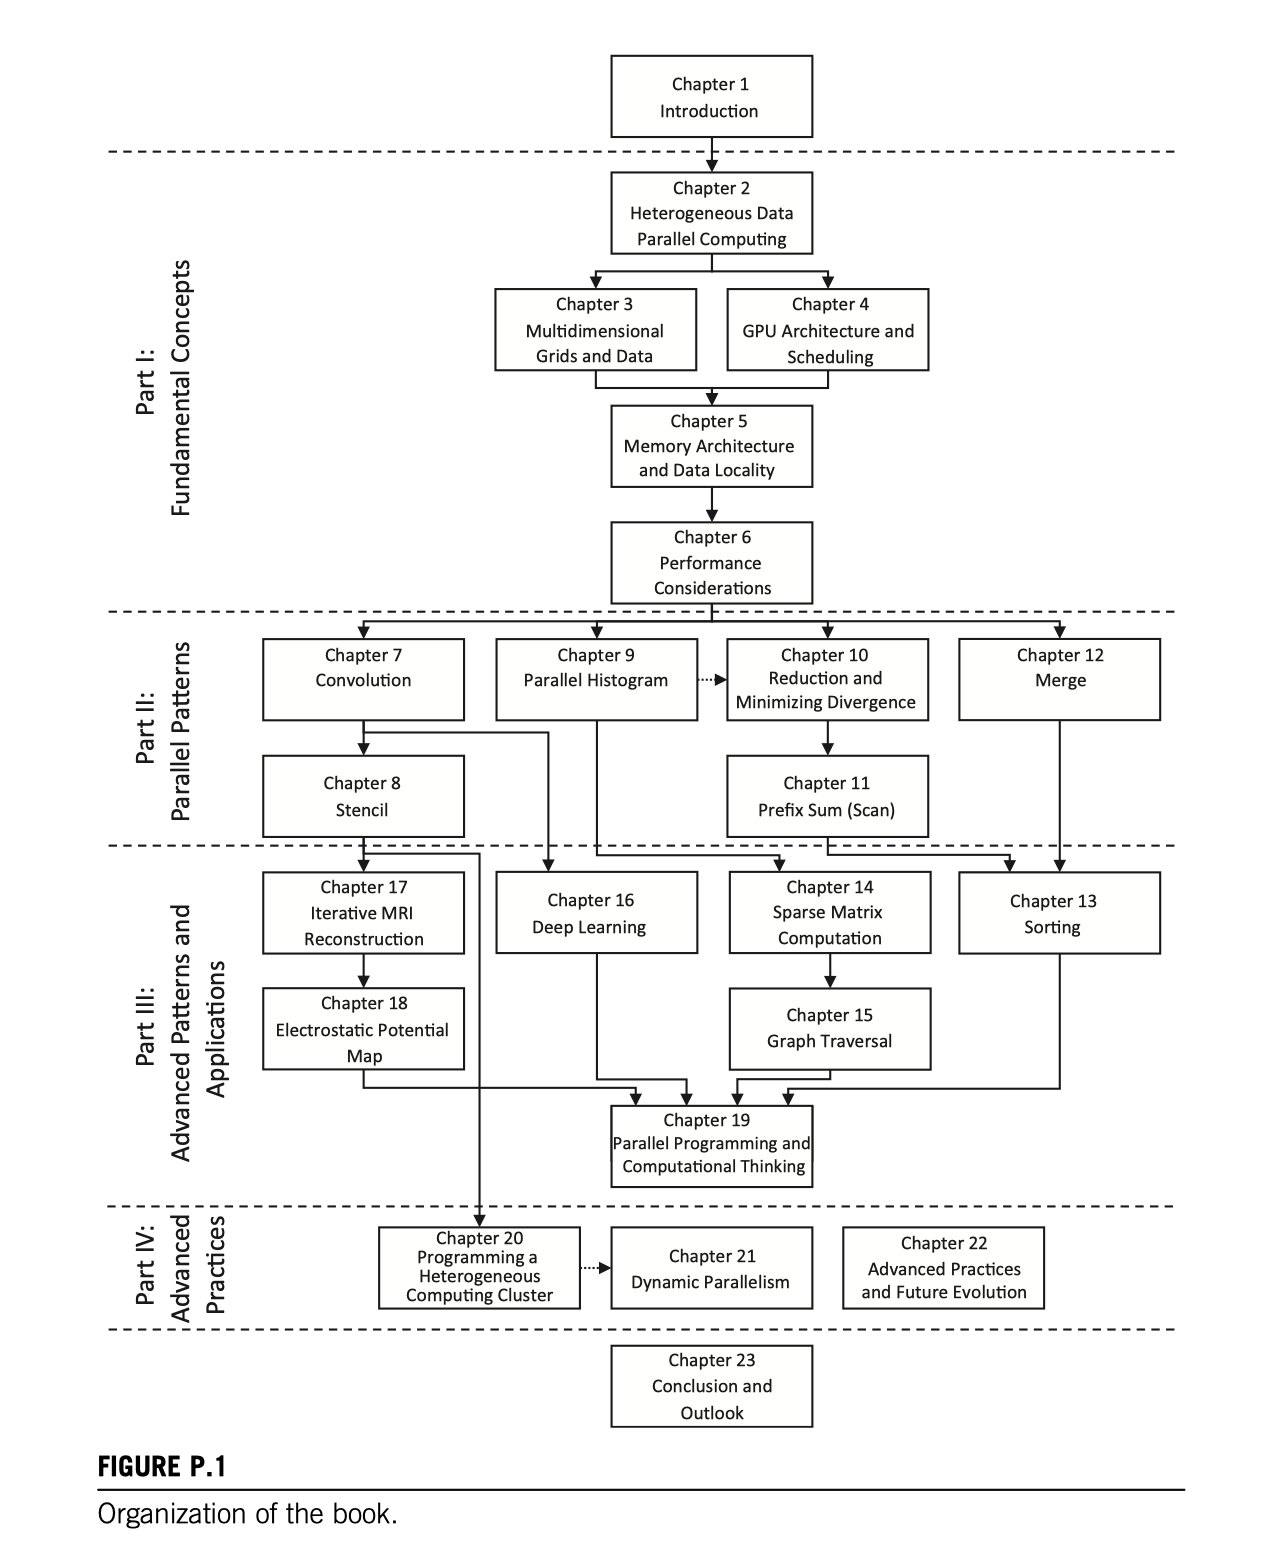
\includegraphics[width=\textwidth]{figs/P.1.png}
\end{figure}

\subsection{如何使用这本书}
我们希望通过本书提供一些教学课程的经验。 自 2006 年以来,我们教授多种类型的课程:一学期课程和一周强化课程。 
最初的 ECE498AL 课程已成为伊利诺伊大学香槟分校的永久课程,称为 ECE408 或 CS483。 
当我们第二次提供 ECE498AL 时,我们开始编写本书的一些早期章节。 
前四章也在 Nicolas Pinto 于 2009 年春天教授的麻省理工学院课程中进行了测试。
从那时起,我们将这本书用于 ECE408 的众多课程以及 Coursera 异构并行编程课程以及 VSCSE 和 PUMPS 暑期学校 。

\subsection{两阶段方法}
书中的大部分章节都设计为每节大约 75 分钟的讲座。 可能需要两节 75 分钟的讲座才能完全讲完的章节
是第 11 章(前缀和(扫描))、第 14 章(稀疏矩阵计算)和第 15 章(图遍历)。 
在 ECE408 中,讲座、编程作业和期末项目是同步进行的,并分为两个阶段。

在第一阶段,即本书的第一部分和第二部分,学生学习基础知识和基本模式,并练习通过指导性编程作业所学到的技能。 
此阶段由 12 章组成,通常需要大约 7 周的时间。 每周,学生都会完成与该周讲座相对应的编程作业。 
例如,第一周,基于第2章的讲座专门讲授基本的CUDA内存/线程模型、CUDA对C语言的扩展以及基本的编程工具。 
讲座结束后,学生可以在几个小时内编写简单的向量加法代码。

接下来的两周包括基于第 3 章到第 6 章的一系列四堂讲座,让学生对 CUDA 内存模型、CUDA 线程执行模型、
GPU 硬件性能特征和现代计算机系统架构有概念性的理解。 
在这两周内,学生们研究矩阵-矩阵乘法的不同实现,他们会看到在此期间其实现的性能如何显着提高。 
在剩下的四个星期中,讲座涵盖了基于第 7 章到第 12 章开发高性能并行应用程序所需的常见数据并行编程模式。
在这几周中,学生完成有关卷积、直方图、约简和前缀和的作业。 在第一阶段结束时,学生应该对并行编程非常熟悉,
并且应该准备好以更少的操作来实现更高级的代码。

在第二阶段(由第三部分和第四部分组成)中,学生在完成涉及加速高级模式或应用程序的最终项目时学习高级模式和应用程序。 
他们还学习了在完成项目时可能会发现有用的高级实践。 尽管我们通常不会在此阶段分配每周的编程作业,
但该项目通常有一个每周里程碑来帮助学生调整自己的节奏。 根据课程的持续时间和形式,教师可能无法涵盖此阶段的所有章节,
可能需要跳过一些章节。 教师还可以选择用客座讲座、论文讨论会或支持最终项目的讲座来代替一些讲座。 
因此,图 P.1 使用箭头来指示章节之间的依赖关系,以帮助教师选择可以跳过或重新排序的章节,以根据其特定上下文定制课程。

\subsection{将它们结合在一起:最终项目}
虽然本书的讲座、实验和章节有助于为学生奠定知识基础,但将学习经验整合在一起的是最终项目。 
最终项目对于整个学期的课程非常重要,因此它在课程中占据显着位置,需要近两个月的时间来重点关注。 
它包含五个创新方面:指导、研讨会、临床、最终报告和研讨会。 
虽然有关最终项目的大部分信息都可以在伊利诺伊州 NVIDIA GPU 教学套件中找到,但我们仍想提供这些方面设计背后的推理。

鼓励学生将他们的最终项目基于代表研究界当前挑战的问题。 为了推动这一过程,
教师应该招募几个计算科学研究小组来提出问题并担任导师。 导师被要求提供一份一到两页的项目规格表,
简要描述申请的重要性、导师希望与学生团队一起完成申请的目标、技术技能(特定类型的数学、物理) 和化学课程),
这是理解和使用应用程序所需的,以及学生可以利用的网络和传统资源列表,以获取技术背景、一般信息和构建块,
以及特定实现的特定 URL 或 FTP 路径 和编码示例。 
这些项目规格表还为学生提供了在其职业生涯后期定义自己的研究项目的学习经验。 
伊利诺伊州-NVIDIA GPU 教学套件中提供了几个示例。

\subsection{设计文档}
一旦学生决定了一个项目并组建了一个团队,他们就需要提交该项目的设计文件。 
这有助于他们在投入项目之前仔细考虑项目步骤。 进行此类规划的能力对于他们以后的职业成功非常重要。 
设计文件应讨论项目的背景和动机、应用程序级目标和潜在影响、最终应用程序的主要特征、
设计概述、实施计划、性能目标、验证计划和验收测试 ,以及项目进度表。

\subsection{项目报告及座谈会}
学生需要提交一份关于其团队主要发现的项目报告。 我们还建议举办全天的班级研讨会。 
在研讨会期间,学生使用与团队规模成比例的演示时段。 
在演示过程中,学生们为了全班同学的利益而突出了他们的项目报告中最好的部分。 
演讲占学生成绩的很大一部分。 每个学生必须单独回答针对该学生的问题,因此可以为同一团队中的个人分配不同的成绩。 
研讨会为学生提供了一个学习如何进行简洁演示的机会,以激励他们的同伴阅读全文。

\subsection{班级竞赛}
2016年ECE408的招生规模远远超过了最终项目进程所能容纳的水平。 结果,我们从期末项目变成了班级竞赛。 
在学期中期,我们宣布了一个竞赛挑战问题。 我们用一个讲座来解释比赛挑战问题以及用于对团队进行排名的规则。 
所有学生提交的内容都会自动评分和排名。 每个团队的最终排名取决于其并行代码的执行时间、正确性和清晰度。 
学生在学期结束时演示他们的解决方案并提交最终报告。 当班级规模导致最终项目不可行时,这种妥协保留了最终项目的一些好处。

\subsection{课程资源}
伊利诺伊州-NVIDIA GPU 教学套件是一个公开资源,其中包含讲座幻灯片和录音、实验作业、
最终项目指南以及为在课堂上使用本书的教师提供的示例项目规范。 此外,我们正在公开基于本书的伊利诺伊州本科生和研究生课程。 
虽然本书为这些课程提供了知识内容,但附加材料对于实现总体教育目标至关重要。

最后,我们鼓励您提交反馈。 如果您有任何改进本书的想法,我们希望收到您的来信。 我们想知道如何改进在线补充材料。 
当然,我们也想知道您喜欢这本书的哪些方面。 我们期待您的回音。
